\section{\textbf{Manufacturing}}\label{sec:4}

	As the simulation (see Section~\ref{sec:3}) proved that the designed circuit works as intended the physical components were assembled in a protoboard for further testing and validation before the final manufacturing \todo{complete with relevant information about final board}. Figure~\ref{fig:proto_h} shows the circuit properly assembled. This circuit's evaluation will be further discussed in Section~\ref{sec:5}.
	
	\todo{TALK ABOUT CIRCUIT PRINTING}
	
	
\begin{figure}
\centering

\begin{subfigure}{.45\columnwidth}
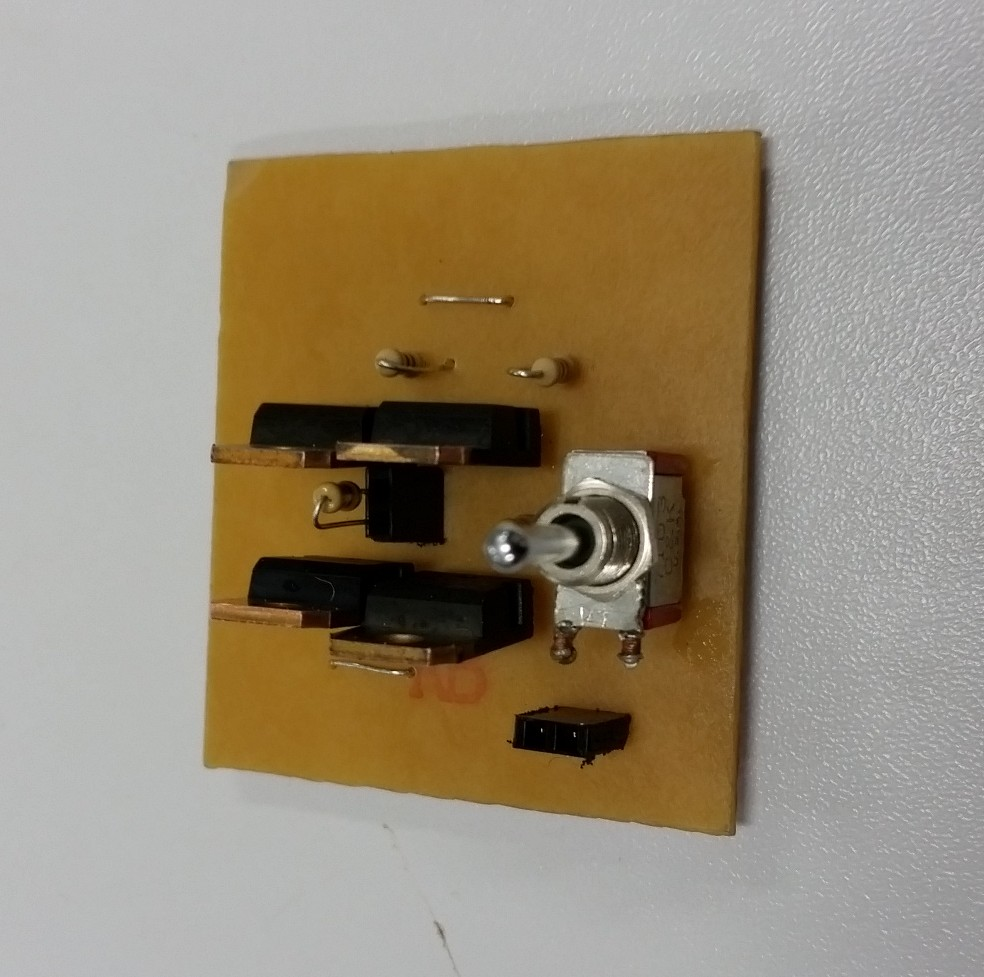
\includegraphics[height=4cm]{img/compontentes4.jpg}
\caption{Components in the PCB.}
\label{fig:pcb_top}
\end{subfigure}
\begin{subfigure}{.45\columnwidth}
\centering
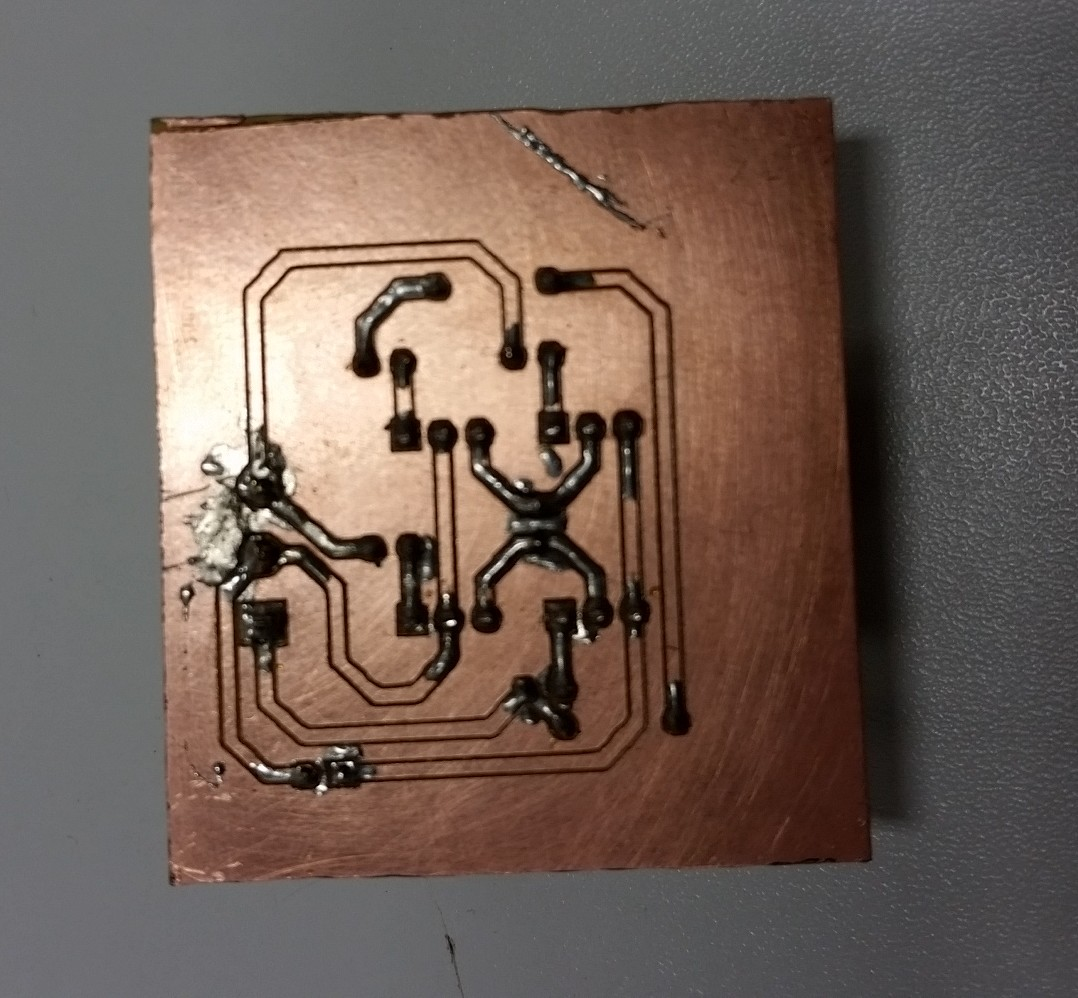
\includegraphics[height=4cm]{img/solda_ja_saiu_da_jaula.jpg}
\caption{Connections in the PCB.}
\label{fig:pcb_bot}
\end{subfigure}
\begin{subfigure}{\columnwidth}
\centering
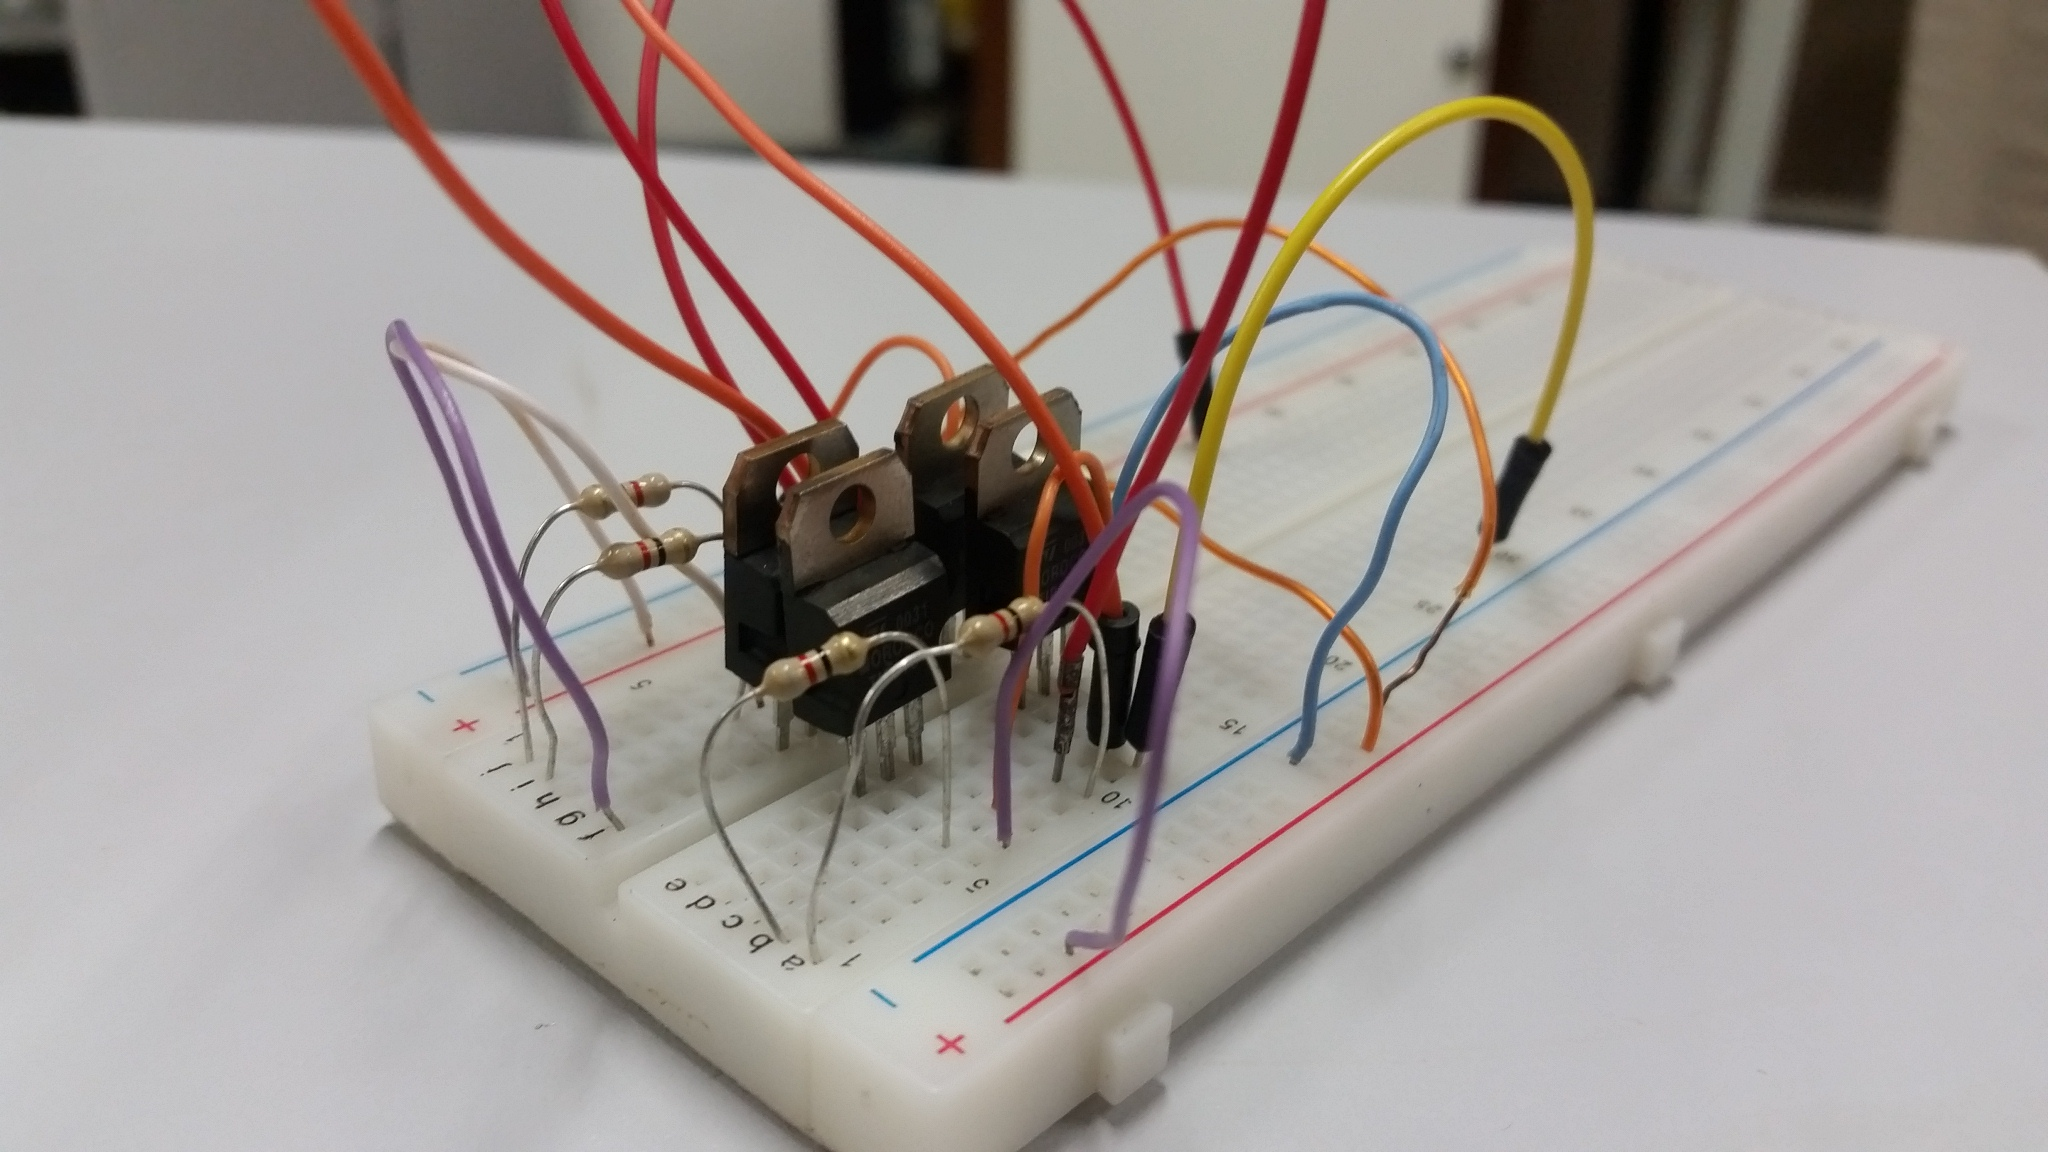
\includegraphics[height=4cm]{img/h_bridge_proto_close.jpg}
\caption{Circuit assembled on a protoboard.}
\label{fig:proto_h}
\end{subfigure}
\caption{Circuit assembling.}
\end{figure}